\chapter{Project Description 
\index{Chapter!Project Description}
\index{Project Description}
\label{Project Description}}
\begin{figure}[H]
  \centering
  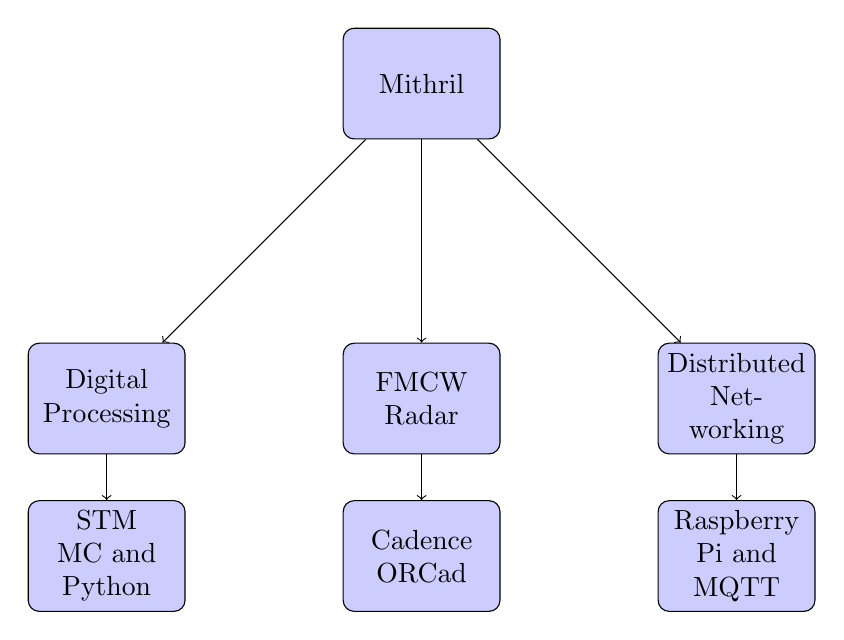
\begin{tikzpicture}[node distance = 2cm, auto]
      % Define block styles
      \tikzstyle{block} = [rectangle, draw, fill=blue!20, 
          text width=5em, text centered, rounded corners, minimum height=4em]
      \tikzstyle{line} = [draw, ->]
  
      % Place nodes
      \node [block] (mithril) {Mithril};
      \node [block, below of=mithril, node distance=4cm] (radar) {FMCW Radar};
      \node [block, left of=radar, node distance=4cm] (processing) {Digital Processing};
      \node [block, right of=radar, node distance=4cm] (networking) {Distributed Networking};
      \node [block, below of=processing, node distance=2cm] (STM) {STM MC and Python};
      \node [block, below of=radar, node distance=2cm] (ORCad) {Cadence ORCad};
      \node [block, below of=networking, node distance=2cm] (pi) {Raspberry Pi and MQTT};
      % Draw edges
      \path [line] (mithril) -- (radar);
      \path [line] (mithril) -- (processing);
      \path [line] (mithril) -- (networking);
      \path [line] (radar) -- (ORCad);
      \path [line] (processing) -- (STM);
      \path [line] (networking) -- (pi);
  \end{tikzpicture}
  \caption{Flowchart of the Mithril system}
  \label{fig:mithril_flowchart}
  \end{figure}
Mithril is a nodal FMCW radar system that incorporates traditional FMCW radar,
digital processing, edge computing, and distributed networking. The initial idea of this 

As can be seen in Figure \ref{fig:mithril_flowchart},
the radar was designed as a standalone PCB in ORCad, digital processing was handled by
STM microcontrollers, and distributed networking is done via Raspberry Pi's and the MQTT protocol.
All of these components were designed, engineered, and interfaced from scratch with a limited budget
of 2000 dollars.

\section{}
The heart of the project is a standalone PCB capable of FMCW radar.